
\documentclass[journal]{IEEEtran}
%\usepackage{lineno}
%\linenumbers
%\usepackage{cite}
\usepackage{comment}
\ifCLASSINFOpdf
  \usepackage[pdftex]{graphicx}
  \graphicspath{pics/}
  \DeclareGraphicsExtensions{.pdf,.jpeg,.png,.jpg}
\else

\fi
\usepackage{amsmath}
\usepackage{siunitx}
\usepackage{geometry}
\usepackage{comment}
\usepackage{float}
\usepackage[caption=false]{subfig}
\usepackage[super]{nth}
\hyphenation{}

\begin{document}
\newgeometry{top=12mm, bottom=12mm, left=12mm, right=12mm}
\title{22051 - Assignment number 1}
\author{\vspace{-2mm}{\normalsize \underline{Group 3} - s194048 Erik Rame (\_ hrs), s194051 Jakob Bernhardt (\_ hrs), s194006 Steffan Kunoy (\_ hrs), \\s186083 Tjark Petersen (\_ hrs)}\vspace{-10mm}}

% make the title area
\maketitle
%\IEEEpeerreviewmaketitle

\section{How finite should it be?}

\subsection{Like a hot knife through a Butterworth}
% Erik
% Jakob
The purpose of this exercise was to construct a bandpass filter which met a set of requirements. These requirements were:
\begin{itemize}
\item Passband from 0.2 to 0.3
\item Stopbands from 0 to 0.1 and 0.4 to 1
\item Ripples are OK if they don't exceed 2 dB
\item The stopband attenuation should be at least -100 dB
\end{itemize}

It was decided to make a Butterworth bandpass filter. MATLAB has a built-in function called 'butter' which returns the transfer function of a Butterworth filter of the specified type, order and cutoff frequency. 
\newline
The requirements meant that we constructed a bandpass Butterworth filter using a higher and lower cutoff frequency of 0.2 and 0.3 respectively. The order was determined by testing the function with different values, and choosing the lowest order where the stopband attenuation was at least -100 dB. The resulting magnitude and phase response of the 12th order Butterworth bandpass filter can be seen in figure \ref{fig:butterband}.

\begin{figure} [H]
    \centering
    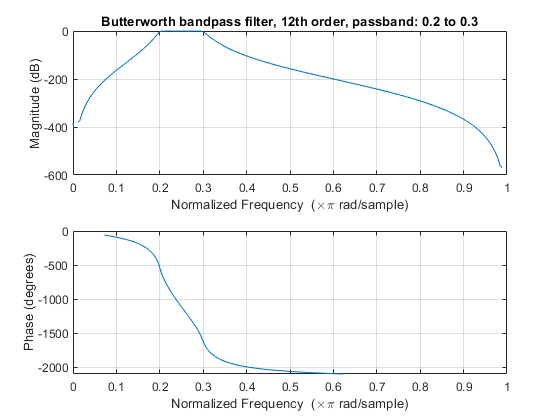
\includegraphics[width=\linewidth]{assignment_02/plots/butterbandfreq.png}
    \caption{Frequency and phase response of a Butterworth bandpass filter that lives up to the given specifications.}
    \label{fig:butterband}
\end{figure}

The next task was to compute and plot the impulse response (figure xx) and the pole-zero plot in the z-plane (figure xx). 
% insert impulse response and pole-zero plot

Using the computed impulse response, we were asked to find the effective length of the impulse response, which is the length (in samples) at which the impulse response decays below 10\% of its maximum. 


\subsection{Shorter and shorter}
% Steffan
For this exercise we were tasked with designing an \textit{ideal} FIR lowpass filter based on the following specifications: 
\begin{itemize}
    \item Pass-band from 0 to 5 kHz with gain of 0 dB. 
    \item Cut-off frequency at one-third the normalized frequency. 
    \item Impulse response is 601 samples long. 
\end{itemize}
From these specifications we can argue that the sampling frequency should be 30 kHz, as the Nyquist frequency would then be 15 kHz, which would correspond to three times the cut-off frequency of 5 kHz. A two-sided frequency response of the filter is shown in Figure \_. 

\section{An equalizer - without buttons}

\subsection{Bass and treble}
% Tjark

\end{document}


